\section{Memory and Disks}
\subsection{Memory Types}
\begin{description}
	\item[Static] memory: Flip-flops or latches used to store bits
	\item[Dynamic] memory: Each cell is a switch (transistor) plus capacitor
	\item[RAM]: Volatile read/write memory
	\item[SRAM]: Static memory
	\item[DRAM]: Dynamic memory
\end{description}

\subsection{Volatility}
\textbf{Volatile memory}
\begin{itemize}
	\item Contents ``forgotten'' when power off
	\item Both SRAM and DRAM are volatile
	\subitem DRAM forgets contents within milliseconds if not refreshed, i.e. contents rewritten	
\end{itemize}
\textbf{Non-volatile memory}
\begin{itemize}
	\item Contents remembered when power off	
	\item \textbf{ROM} - Read only memory
	\item \textbf{EPROM} - Erasable Programmable ROM
	\item \textbf{EEPROM} - Electronically Erasable PROM
	\item \textbf{Flash} - New EEPROM
\end{itemize}

\begin{note}{When do use powers of 2 or 10}
	\begin{itemize}
		\item \textbf{Main Memory} capacity, always 	based on powers of 2
		\subitem $1GB=1024\times1024\times1024 bytes = 2^{30} bytes$
		\item \textbf{Hard Disks}, manufacturers base sizes on powers of 10
		\subitem $1GB = 1000\times1000\times1000 bytes=10^9bytes$
		\subitem Operating Systems base sizes on powers of 2
		\item \textbf{Data Speeds (transfer rates)} based on powers of 10
		\subitem $1Gbps = 10^9 bits per second$
	\end{itemize}
\end{note}

\subsection{Kibibytes, Mebibytes}
\begin{itemize}
	\item Kilo-, mega-, giga- prefixes mean powers of 10 in SI units
	\item 1 \textbf{kibibyte} = 1KiB = 1024 bytes
	\item 1 \textbf{mebibyte} = 1MiB = 1024 KiB
	\item 1 \textbf{gibibyte} = 1GiB = 1024 MiB	
\end{itemize}

\subsection{Types of DRAM}
\begin{itemize}
	\item Bits stored as charge on capacitor, not in flip-flops
	\item Cells are smaller, so can pack more bits on a chip than static memory
	\item Fast Page Mode (FPM DRAM)
	\item Extended Data Out (EDO DRAM)
	\item Synchronous DRAM (SDRAM)
	\item Rambus DRAM (RDRAM)
	\item Double Data Rate DRAM (DDR DRAM) 1, 2, 3, and 4	
\end{itemize}

\subsection{Cache Memory}
\begin{itemize}
	\item CPUs are faster than main memory
	\item Small amount of very fast memory combined with larger slower memory
	\item Most commonly used memory words kept in cache
	\item Three levels, each lower is progressively slower but larger	
\end{itemize}

\subsection{Magnetic Disks}
\begin{itemize}
	\item Rotating \textbf{platters} with magnetised coating
	\item Data stored magnetically in circular \textbf{tracks}
	\item Read/write \textbf{heads} float above platter surfaces
	\item Usually use both sides of platters	
\end{itemize}

\subsubsection{Sectors and Tracks}
\begin{figure}
	\centering
	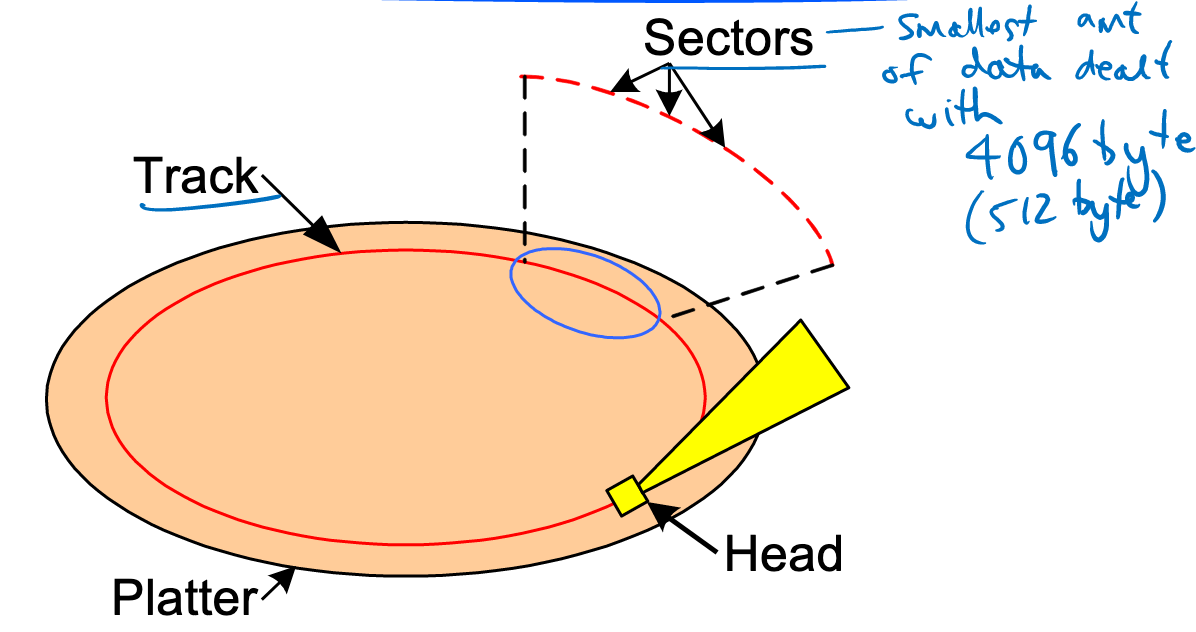
\includegraphics[width=0.8\linewidth]{disk}
	\caption{The break up of what a disk is}
\end{figure}

\subsubsection{Cylinders}
\begin{itemize}
	\item Set of tracks at a given radial position
	\item Number of tracks in cylinder = 2 x number of platters
\end{itemize}

\subsubsection{Sectors}
\begin{itemize}
	\item Tracks divided into fixed-length sectors
	\subitem Smallest data unit, i.e. must read/write a whole sector at a time
	\item Sector consists of: Preamble, Data, Error correction codes (ECCs), Inter-sector gap
	\item About 85\% of disk capacity usable by operating system	
\end{itemize}

\subsubsection{Access Time}
\begin{itemize}
	\item \textbf{Access Time} = seek time + rotational latency + transfer time
	\item \textbf{Seek time} - time to move heads to right cylinder
	\item \textbf{Rotational latency} - time to wait for sector to arrive under head
	\item \textbf{Transfer time} - Time for sector to pass under	
\end{itemize}

What's the average access time for a hard dick which rotates at 7200rpm and has an edge-to-edge seek time of 10ms? (Assume that seek time is proportional to the number of tracks to seek)
\begin{align*}
	\text{Avg Access Time} &= \text{Avg seek time} + \text{Avg rotational}\\
	&= \frac{\text{e-to-e seek}}{3} + \frac{\text{rot time}}{2}\\
	&= \frac{10}{3} + \frac{1/120}{2}\\
	&= 7.5ms
\end{align*}


